\documentclass[a4paper]{article}
\usepackage[russian]{babel}
\usepackage[left=2cm, right=2cm, top=2cm, bottom=2cm]{geometry}
\usepackage{graphicx}
\usepackage{hyperref}
\hypersetup{
    colorlinks,
    citecolor=black,
    filecolor=black,
    linkcolor=black,
    urlcolor=black
}
\usepackage[utf8]{inputenc} 
\usepackage[T1]{fontenc}
\usepackage{amsmath}
\usepackage{bookmark}
\usepackage[skins]{tcolorbox}
\usepackage{amsfonts}
\usepackage{amsthm}
\usepackage{indentfirst}
\usepackage{booktabs}
\usepackage{tabularx}

\newcommand{\nicecolor}{blue!50!violet!50}
\newcommand{\norm}[1]{\left \lVert #1 \right \rVert}
\newtheorem{definition}{Определение}

\author{Берлет Максим гр. 3384 \\ Вариант 2.}
\title{Домашняя работа 2. \\ Операторная норма.}
\date{}

\begin{document}

\maketitle
\pagebreak

\tableofcontents
\pagebreak

\section{Условие}
\begin{tcolorbox}[title=Условие задания, colframe=\nicecolor, fonttitle=\bfseries]
    Линейный оператор $\mathcal{A} : \mathbb{R}^4 \rightarrow \mathbb{R}^4$ задан матрицей $A \in \mathbb{R}_{4x4}$ \\
    Требуется вычислить:
        \begin{itemize}
            \item норму оператора $\mathcal{A}$ в пространствах $l_{4}^{1}$, $l_{4}^{\infty}$ и предъявить векторы, на которых достигается норма.
            \item норму оператора $\mathcal{A}^{-1}$ в пространствах $l_{4}^{1}$, $l_{4}^{\infty}$ и предъявить векторы, на которых достигается норма.
            \item число обусловленности $\mu(A)$ оператора в пространствах $l_{4}^{1}$, $l_{4}^{\infty}$.
            \item показать, что матрица $G = A^{*}A$ положительно определенная и найти её собственные числа и собственны вектора.
            \item норму оператора $\mathcal{A}$ в пространстве $l_{4}^{2}$.
        \end{itemize}
    Задание на пятерку: 
    \begin{itemize}
        \item решить систему $Ax = b$ методом итераций.
        \item сравнить результат с точным решением.
    \end{itemize}
    \tcblower
    
    Матрица задающая оператор:
    $
    A = \begin{bmatrix}
    \frac{333}{11} & \frac{288}{11} & \frac{18}{11} & \frac{270}{11} \\\\
    \frac{819}{22} & \frac{1305}{22} & \frac{-315}{11} & \frac{324}{11} \\\\
    \frac{-1257}{44} & \frac{-1773}{44} & \frac{453}{22} & \frac{-315}{11} \\\\
    \frac{-81}{44} & \frac{-549}{44} & \frac{351}{22} & \frac{108}{11} \\\\
    \end{bmatrix}
    $
\end{tcolorbox}
\pagebreak

\section{Норма оператора \texorpdfstring{$A$}{}}

\begin{definition} 
    Нормой линейного оператора $\mathcal{A}: X \rightarrow Y$ называется такое число \\ $\norm{\mathcal{A}} = sup\{\norm{ \mathcal{A} x}: \norm{x} \le 1\}$     
\end{definition}

Если говорить просто, то нормой оператора будет максимальный коэффициент растяжения пространства. Это легко проиллюстрировать на единичной окружности.
\begin{figure}[h]
    \centering
    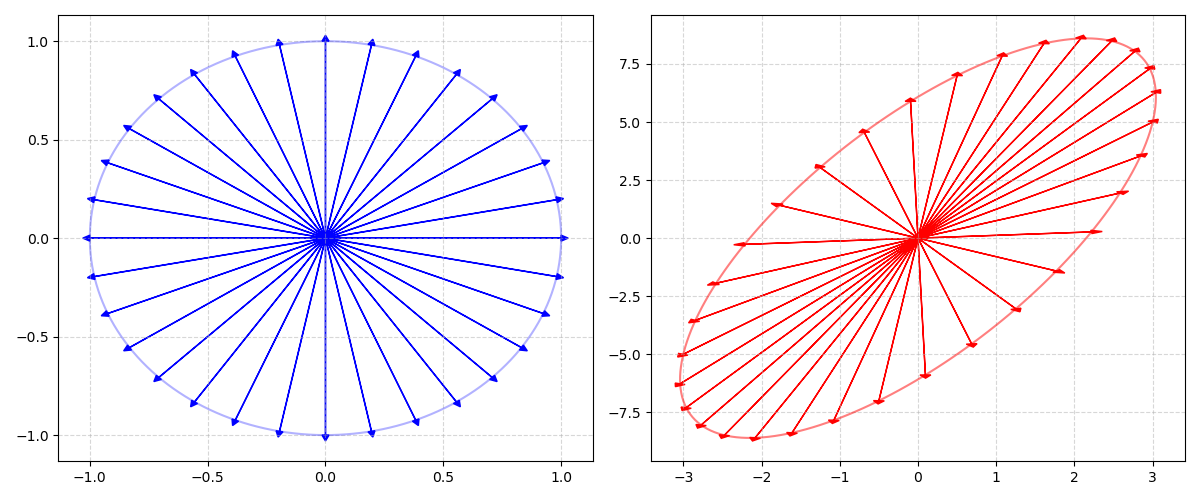
\includegraphics[width=10cm]{utils/Figure_1.png}    
    \caption{Изображение линейного преобразования}
\end{figure}

На левом графике изображена единичная окружность, на правом изображен эллипс, полученный с помощью применения некого линейного оператора к каждому вектору с левого графика.
Кроме того, видно, что оператор растягивает вектора (увеличивает их длину) в доль одного наравления больше, чем вдоль другого, так норма этого оператора будет показывать самое большое растяжение единичного вектора.

На практике никто не использует определение для вычисления нормы оператора. Так как норма оператора всегда индуцирована нормой вектора, возникает множество разных норм из разных геометрий пространства.
Наиболее часто используемые: $l_{n}^{1}$ - Манхэттенская геометрия, $l_{n}^{2}$ - Евклидова геометрия, $l_{n}^{\infty}$ - геометрия Чебышёва.

\subsection{Норма в \texorpdfstring{$l_{4}^{1}$}{}}
\begin{definition} нормой $x \in l_{n}^{1}$ называется
    $\norm{x}_1 = \sum_{k=1}^{n}|x_k|$
\end{definition}
Пусть $x \in l_{4}^{1}$ тогда

\begin{align*}
\norm{Ax}_1 = \sum_{k=1}^{4} |(a_k, x)| = \sum_{k=1}^{4} |\sum_{j=1}^{4} a_{kj} x_j| \le
& \sum_{k=1}^{4} \sum_{j=1}^{4} |a_{kj} x_j| = \sum_{j=1}^{4} |x_j| \sum_{k=1}^{4} |a_{kj}|
& \le  \sum_{j=1}^{4} |x_j| \max\limits_{j} \sum_{k=1}^{4} |a_{kj}| \\
& = \max\limits_{j} \sum_{k=1}^{4} |a_{kj}| \cdot \norm{x}_1 = \norm{A}_1\norm{x}_1
\end{align*}

Так как максимум берется по строке, то выбирается столбец с самой большой суммой элементов, а значит, чтобы найти вектор, на котором достигается эта норма и вектор должен удовлетворять условию по определению $\norm{x} \le 1$.
Максимум достигается при норме равной 1. А так как умножение матрицы на вектор это линейная комбинация столбцов матрицы с весами из вектора $x$, то нужно взять тот столбец, у которого норма больше всех.

Вычислим норму для заданного оператора с помощью библиотеки \emph{numpy} для \emph{python}.

$\norm{\mathcal{A}}_{1} = 138.27$ - это сумма элементов первого столбца, а значит достигается эта норма на стандартном базисном векторе $e_1=(1, 0, 0, 0)^T$.

\subsection{Норма в \texorpdfstring{$l_{4}^{\infty}$}{}}
\begin{definition} нормой $x \in l_{n}^{\infty}$ называется
    $\norm{x}_\infty = \max\limits_{k}{|x_k|}$
\end{definition}

Пусть $x \in l_{4}^{\infty}$ тогда

\begin{align*}
\norm{Ax}_{\infty} = \max\limits_{i}{|(a_{i}, x)|} = \max\limits_{i} |\sum_{j=1}^{4} a_{ij}x_{j} | \le \max\limits_{i} \sum_{j=1}^{4}|a_{ij} x_j| \le  \max\limits_{i} \sum_{j=1}^{4}|a_{ij}| \norm{x}_{\infty} = \norm{A}_\infty \norm{x}_\infty
\end{align*}
 
Вычислим норму для заданного оператора с помощью библиотеки \emph{numpy} для \emph{python}.
$\norm{A}_\infty = 154.64$ - это сумма элементов первой строки.

Так как в данной норме максимум берется по строке, значит нужно максимизировать $(a_i, x) = \sum_{j=1}^{4}a_{ij}x_j$.
При этом $\norm{x}_\infty = 1$. То есть мы хотим, чтобы все $a_{ij}$ складывались друг с другом, а не вычитались, тогда возьмем $x_j = sign(a_{ij})$ и получим
$(a_i, x) = \sum_{j=1}^{4}a_{ij} \cdot sign(a_{ij}) = \sum_{j=1}^{4}|a_{ij}|$.
Таким образом данная норма достигается на векторе $x = (sign(a_{ij}))$, где $i = argmax_{k}{\sum_{j=1}^{4}|a_{kj}|}$


\section{Норма оператора \texorpdfstring{$\mathcal{A}^{-1}$}{}}
Найдем ядро оператора, оператор обратим, если ядро состоит только из нуля. Это можно сделать несколькими способами, воспользуемся SVD разложением, которое можно применять для любой прямоугольной матрицы. 

$
A = \begin{bmatrix}
\frac{333}{11} & \frac{288}{11} & \frac{18}{11} & \frac{270}{11} \\\\
\frac{819}{22} & \frac{1305}{22} & \frac{-315}{11} & \frac{324}{11} \\\\
\frac{-1257}{44} & \frac{-1773}{44} & \frac{453}{22} & \frac{-315}{11} \\\\
\frac{-81}{44} & \frac{-549}{44} & \frac{351}{22} & \frac{108}{11} \\\\
\end{bmatrix} \approx \\
\approx \begin{bmatrix}
-0.39 & 0.65 & -0.61 & -0.22 \\
 -0.73 & -0.26 & -0.04 & 0.63 \\
 0.55 & -0.01 & -0.58 & 0.61 \\ 
 0.09 & 0.71 &  0.54 & 0.44 \\
\end{bmatrix} \cdot
\begin{bmatrix}
 110.29 & 0 & 0 & 0 \\
 0 & 27.55 & 0 & 0   \\
 0 & 0 & 8.08 & 0  \\
 0 & 0 & 0 & 2.40 \\
\end{bmatrix} \cdot
\begin{bmatrix}
 -0.50 & -0.70 & 0.30 & -0.42 \\
 0.32 & -0.26 & 0.72 & 0.56 \\
 -0.54 & -0.21 & -0.39 & 0.72 \\
 0.72 & 0.63 & 0.49 & 0.01 \\
\end{bmatrix}
$

Из диагональной матрицы в центре видно, что в ядре оператора лежит только 0, потому что нет ни одного нулевого сингулярного числа, которому бы соответствовал правый сингулярный вектор.
А значит существует обратный оператор к оператору $\mathcal{A}$ найдем его.

$
A^{-1} = \begin{bmatrix}
 \frac{31}{297} & \frac{-136}{891} & \frac{-34}{297} & \frac{-122}{891} \\\\
 \frac{-1}{22} & \frac{103}{594} & \frac{17}{99} & \frac{28}{297} \\\\
 \frac{1}{1188} & \frac{431}{3564} & \frac{91}{594} & \frac{73}{891} \\\\
 \frac{-47}{1188} & \frac{-17}{3564} & \frac{-31}{594} & \frac{56}{891} \\\\
\end{bmatrix}
$

\subsection{Норма в \texorpdfstring{$l_{4}^{1}$}{}}
Определение нормы аналогично определению выше. $\norm{A^{-1}}_1 = 0.49$.
Интересный результат, это значит, что данный оператор является сжимающим.
\subsection{Норма в \texorpdfstring{$l_{4}^{\infty}$}{}}
Определение нормы аналогично определению выше. $\norm{A^{-1}}_\infty = 0.51$.
\pagebreak

\section{Число обусловленности оператора \texorpdfstring{$A$}{}}
Рассмотрим задачу вида: $Ax = b$, в реальной жизни на практике мы никогда не будем иметь идеально точный вектор отклика $b$, он будет иметь некоторый шум, а значит задача становится такой:
$Ax = b + \Delta{b}$. То же самое можно сказать и про оператор и про неизвестный вектор. В итоге, имеем следующее зашумленное уравнение
$(A + \Delta{A})(x + \Delta{x}) = b + \Delta{b}$, где $\Delta{A}\Delta{b} \approx 0$. Выразим ошибку: $\Delta{x} = -A^{-1}\Delta{A}x + A^{-1}\Delta{b}$. Посчитаем норму ошибки(её величину):
$\norm{\Delta{x}} = \norm{A^{-1}\Delta{b} - A^{-1}\Delta{A}x} \le \norm{A^{-1}\Delta{b}} + \norm{A^{-1}\Delta{A}x} \le \norm{A^{-1}}\norm{\Delta{b}} + \norm{A^{-1}}\norm{\Delta{A}}\norm{x}$.
При этом $\norm{Ax} = \norm{b} \le \norm{A}\norm{x} \Rightarrow \norm{x} \ge \frac{\norm{b}}{\norm{A}}$.
Отсюда получаем: $\norm{A^{-1}}\norm{\Delta{b}}\frac{\norm{A}\norm{b}}{\norm{b}\norm{A}} + \norm{A^{-1}}\norm{\Delta{A}}\norm{x}\frac{\norm{A}}{\norm{A}} \le \norm{A}\norm{A^{-1}}\frac{\norm{\Delta{b}}}{\norm{b}}\norm{x} + \norm{A}\norm{A^{-1}}\frac{\norm{\Delta{A}}}{\norm{A}}\norm{x} = \norm{A}\norm{A^{-1}}(\frac{\norm{\Delta{A}}}{\norm{A}} + \frac{\norm{\Delta{b}}}{\norm{b}})\norm{x}$.
В итоге, имеем следующее неравенство, связывающее относительны погрешности: $\frac{\norm{\Delta{x}}}{\norm{x}} \le \mu(\frac{\norm{\Delta{A}}}{\norm{A}} + \frac{\norm{\Delta{b}}}{\norm{b}})$, где $\mu = \norm{A}\norm{A^{-1}}$ - число обусловленности матрицы $A$.

\subsection{\texorpdfstring{$\mu(A)$}{} в \texorpdfstring{$l_{4}^{1}$}{}}
Воспользуемся ранее вычисленными значениями норм $\mu(A) = \norm{A}_1\norm{A^{-1}}_1 = 138.27 \cdot 0.49 \approx 67.75$ 

\subsection{\texorpdfstring{$\mu(A)$}{} в \texorpdfstring{$l_{4}^{\infty}$}{}}
Воспользуемся ранее вычисленными значениями норм $\mu(A) = \norm{A}_\infty\norm{A^{-1}}_\infty = 154.64 \cdot 0.51 \approx 78.87$ 

\subsection{Смысл обусловленности матрицы задающей линейное преобразование}
Для понимания сути обусловленности перепишем полученное выше неравенство
$\frac{\norm{\Delta{x}}}{\norm{x}} \le \mu (\frac{\norm{\Delta{A}}}{\norm{A}} + \frac{\norm{\Delta{b}}}{\norm{b}})$
То есть относительная ошибка решения системы не превосходит константы умноженной на сумму относительных ошибок условия системы.
Иными словами число обусловленности показывает, как сильно будет изменяться решение при изменении исходных данных.

Проверим это руками: возьмем за вектор $b = (1, 2, 3, 4)^{T}$, а за ошибку $\Delta{b} = \frac{1}{10}(1,1,1,1)^{T}$, оператор менять не будем.
Решим $Ax = b$, получим в качестве решения $x \approx (-1.09,\ 1.19,\ 1.03,\ 0.05)^{T}$. Решим $A\tilde{x} = b + \Delta{b}$, получаем в качестве решения $\tilde{x} \approx (-1.12,\ 1.23,\ 1.07,\ 0.04)^{T}$.
Так как оператор не зашумлен, то неравенство упрощается в следующее: $\frac{\norm{\Delta{x}}}{\norm{x}} \le \mu \frac{\norm{\Delta{b}}}{\norm{b}}$. 

Рассчитаем относительную ошибку $\frac{\norm{\Delta{x}}}{\norm{x}} = \norm{x - \tilde{x}} \le \mu \frac{\norm{\Delta{b}}}{\norm{b}}$.
Получаем $0.03 \le 2.47$, что является правдой, так как справа стоит верхняя грань ошибки, которая расположена вдоль направления самого большого сингулярного вектора.
\pagebreak

\section{Норма оператора \texorpdfstring{$A$}{} в \texorpdfstring{$l_{4}^{2}$}{}}
Норма в пространстве $l_{4}^{2}$ является довольно трудно вычислимой нормой по сравнению с предыдущими, ведь она требует вычисления сингулярных чисел, а значит и сингулярного разложения, что уже довольно дорого по количеству операций ($O(n^3)$ для квадратных матрицы), нежели просто сложить числа и найти самое большое среди всех.
Зато является часто используемой нормой, например, в методах оптимизации спектральная норма матрицы Гессе показывает локальную кривизну, в методе Гаусса-Зейделя обеспечивает сходимость при определенном условии.
\subsection{Положительная определенность матрицы \texorpdfstring{$G = A^{*}A$}{}}
Проверим положительную определенность матрицы с помощью критерия Сильвестра: \\ матрица положительно определенна $\Leftrightarrow$ все угловые миноры положительны.

$
\Delta_4 = \begin{vmatrix}
\frac{333}{11} & \frac{288}{11} & \frac{18}{11} & \frac{270}{11} \\\\
\frac{819}{22} & \frac{1305}{22} & \frac{-315}{11} & \frac{324}{11} \\\\
\frac{-1257}{44} & \frac{-1773}{44} & \frac{453}{22} & \frac{-315}{11} \\\\
\frac{-81}{44} & \frac{-549}{44} & \frac{351}{22} & \frac{108}{11} \\\\
\end{vmatrix} \approx 59049
$

$
\Delta_3 = 
\begin{vmatrix}
\frac{333}{11} & \frac{288}{11} & \frac{18}{11} \\\\
\frac{819}{22} & \frac{1305}{22} & \frac{-315}{11}\\\\
\frac{-1257}{44} & \frac{-1773}{44} & \frac{453}{22}  \\\\
\end{vmatrix} \approx 3711.27
$

$
\Delta_2 = 
\begin{vmatrix}
\frac{333}{11} & \frac{288}{11} \\\\
\frac{819}{22} & \frac{1305}{22} \\\\
\end{vmatrix} \approx 821.05
$

$
\Delta_1 = 
\begin{vmatrix}
\frac{333}{11}
\end{vmatrix} \approx 30.27
$


\subsection{\texorpdfstring{$\mu(A)$}{} в \texorpdfstring{$l_{4}^{2}$}{}}
Для вычисления числа обусловленности оператора в пространстве $l_{4}^{2}$, необходимо понять, как вычисляется операторная норма, порожденая векторной нормой этого пространства.
$ \norm{A}_2 = \max\limits_{\norm{x}_2 = 1}{\norm{Ax}_2} $, возведем обе части в квадрат.
$ \norm{A}_{2}^{2} = \max\limits_{\norm{x}_2 = 1}{\norm{Ax}_{2}^{2}} = \max\limits_{\norm{x}_2 = 1}{(Ax)^T(Ax)} = \max\limits_{\norm{x}_2 = 1}{x^T(A^TA)x} = \max\limits_{\norm{x}_2 = 1}{x^TGx} = \lambda_{max}x^Tx = \lambda_{max}\norm{x}_{2}^2 = \lambda_{max}$.
Таким образом максимум достигается, когда $x$ - собственный вектор, соответствующий максимальному собственному числу матрицы $G = A^*A$(в вещественном случае $G = A^TA$).
А корнем из этого числа для нахождения нормы, а не квадрата нормы, будет сингулярное число исходной матрицы(корень мы можем спокойно брать из-за положительной определенности матрицы $G$).

Вычислим собственные числа и собственные векторы $G$.
Cобственные числа:
$\lambda_1 \approx 5.78,\ \lambda_2 \approx 65.29,\ \lambda_3 \approx  759.21,\ \lambda_4 \approx  12162.84$.

Собственные векторы:
$v_1 \approx (0.60,\ -0.54,\ -0.32,\ -0.50)^T,\ v_2 \approx (-0.63,\ -0.21,\  0.26,\ -0.70)^T,\ v_3 \approx (-0.49,\ -0.39,\ -0.72,\ 0.30)^T,\ v_4 \approx (-0.01,\ 0.72,\ -0.56,\ -0.42)^T$

Для определения нормы возьмем корень из самого большого собственного числа $\norm{A} = \sqrt{\lambda_{max}} = \sigma_{max}(A) \approx \sqrt{12162.84} \approx 110.29$.

Норма обратного оператора ищется проще, так как при обращении оператора его сингулярные числа просто становятся обратными, то максимальное сингулярное число становится обратным к минимальному сингулярному числу исходного оператора.
То есть $\sigma_{max}(A^{-1}) = \frac{1}{\sigma_{min}(A)} \approx \frac{1}{5.78} \approx 0.17$.

Так число обусловленности оператора в пространстве $l_{4}^{2}$ равно $\mu(A) = \norm{A}_2\norm{A^{-1}}_2 \approx 110.29 \cdot 0.17 \approx 18.75$.
\pagebreak

\section{Задание на пятерку}
\subsection{Описание метода итераций}

Пусть линейный непрерывный оператор $\mathcal{A}: X \rightarrow X$, причем $X$ - Банахово пространство. Если уравнение $Ax = b$ при перезаписи $(I - B)x = b$ допускает оценку $\norm{B} = q < 1$ ($B$ - сжимающее отображение), то последовательность
$x_{n+1} = b + Bx_n$ сходится к $x^*$ - решение исходного уравнения.

По условию задания $B = G^{-1}$, $b = (\frac{1}{2},\ \frac{1}{3},\ \frac{1}{4},\ \frac{1}{5})^T$, $x_0 = (1, 1, 1, 1)^T$.
\subsection{Результат применения метода итераций и сравнение с точным решением}
Для применения нужно удостовериться, что $\norm{B} = q < 1$. Вычислим $\norm{B}_1 \approx 0.17$, а значит можно спокойно использовать метод.
\begin{table}[ht]
    \centering
    \begin{tabularx}{\textwidth}{X||X|X|X}
    решение & $x_5$ & $x_{10}$ & $x^*$ \\
    \midrule
    значение & (0.4979654,\ 0.33919278,\ 0.25599548,\ 0.19703883) & (0.49801044,\ 0.33914479,\ 0.25595833,\ 0.19703857) & (0.49801045,\ 0.33914478,\ 0.25595833,\ 0.19703857) \\
    \end{tabularx}
    \caption{Сравнение решений}
\end{table}

Значения в таблице 1 были приведены без ручного округления. Заметим, что некоторые числа начинают совпадать с точным решением уже на 5 итерациях, то есть метод довольно быстро сходится. При 10 же итерациях мы имеем почти полное совпадение всех цифр после запятой.

\begin{figure}[ht]
    \centering
    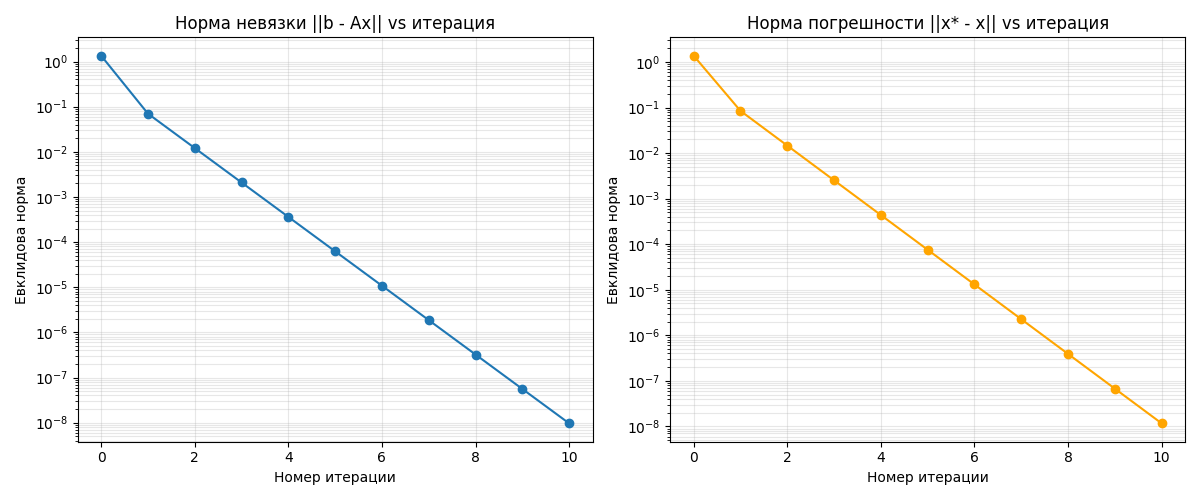
\includegraphics[width=17cm]{utils/Figure_2.png}
    \caption{Графики оценки эффективности метода итераций}
\end{figure}

На рисунке 2 графики изображены в полулогарифмическом масштабе, то есть y в логарифмическом масштабе, а x в линейном.
Видно, что как норма ошибки, так и норма невязки убывают линейно в таком масштабе, а значит, что на практике они убывают с экспоненциальной скоростью.

\pagebreak

\section{Вывод}
    В ходе работы были применены знания об операторных нормах. Всякая норма линейного оператора порождена векторной нормой того же пространства. Были проведены вычисления некоторых операторных норм.
Было вычислено число обусловленности матрицы, задающей линейный оператор, проверено неравенство связывающее относительную ошибку решения с относительной ошибкой исходных данных.
Для решения линейной системы был использован метод итераций, который сошелся за 10 итераций максимально близко к точному решению. Построены графики нормы ошибок, нормы невязок в полулогарифмическом масштабе.
Метод итераций сходится с экспоненциальной скоростью.

\end{document}